\documentclass[12pt]{article}
\usepackage{url,amsmath,setspace,amssymb}
\usepackage{listings}

\usepackage{tcolorbox}
\usepackage{tikz}
\usepackage{xcolor}
\usepackage{multicol}
\usepackage{graphicx}
\usepackage{enumitem}
\usepackage{subcaption}

\usepackage{color}
\def\R{\color{red}}
\def\B{\color{blue}}

\usepackage{listings}
\usepackage{caption}
\usepackage[style=numeric, backend=biber]{biblatex}
\usepackage[colorlinks=true, allcolors=blue]{hyperref}  % Imposta il colore dei link su blu
\usepackage{url}
\addbibresource{bib.bib}



%**********************************************
%* Leave the page configuration as is
\setlength{\oddsidemargin}{.25in}
\setlength{\evensidemargin}{.25in}
\setlength{\textwidth}{6.25in}
\setlength{\topmargin}{-0.4in}
\setlength{\textheight}{8.5in}

\newcommand{\heading}[5]{
\renewcommand{\thepage}{#1-\arabic{page}}
\noindent
\begin{center}
	\framebox[\textwidth]{
	\begin{minipage}{0.9\textwidth} \onehalfspacing
	{\bf #1} \hfill #2

	{\centering \Large #5

	}\medskip
	{#3 \hfill #4}
	\end{minipage}
}
\end{center}
}

%**********************************************


%**********************************************
%* Some more or less useful stuff

\lstnewenvironment{myalgorithm}[1][] %defines the algorithm listing environment
{
   % \captionsetup{labelformat=algocaption,labelsep=colon}
    \lstset{ %this is the stype
        mathescape=true,
        frame=none,
        numbers=none,
        basicstyle=\normalsize,
        keywordstyle=\color{black}\bfseries\em,
        keywords={,input, output, return, datatype, function, in, if, else, foreach, while, begin, end, },
        numbers=left,
        xleftmargin=.04\textwidth,
        #1 % this is to add specific settings to an usage of this environment (for instance, the caption and referable label)
    }
}
{}





\newtcolorbox{alert}[1]{
colback=red!5!white, colframe=red!75!white,fonttitle=\bfseries, title = #1}

\newtcolorbox{commentbox}[1]{
colback=black!5!white, colframe=black!75!white,fonttitle=\bfseries, title = #1}
%**********************************************



\newcommand{\handout}[5]{\heading{#1}{#2}{#3}{#4}{#5}}


%* The document starts here
\begin{document}


%**********************************************
% Edit the input values to the \handout command 
%**********************************************

\handout{Small Project}{Submission Date}{Alessandro Castelli}{12246581}{Study on Solar Energy Production}

\section{Introduction}
In recent years, there has been a growing interest in renewable energies, at the expense of the use of fossil fuels. This shift in perspective reflects an increasing awareness of environmental impacts and the need for transitions towards more sustainable energy sources.
\\
Among the many options available, solar energy emerges as one of the most widely adopted solutions. Its popularity stems from its clean and sustainable nature, based on the abundance of solar radiation. This energy source plays a crucial role in reducing greenhouse gas emissions and contributing to the transition towards a greener and eco-friendly energy landscape.
\\
The implementation of solar energy not only provides environmental benefits but also presents economic and technological opportunities. Solar technologies are constantly evolving, making the utilization of this resource more cost-effective and efficient. Investing in renewable energies, including solar energy, represents a crucial step towards a more sustainable and resilient energy future.
\\
In this context, the main objective will be to develop predictive models capable of estimating energy generation levels based on various assumptions. The subsequent document will focus on this theme, proposing modifications, improvements, and further insights.

\section{Outline}
The project presented in the following pages focuses on the prediction of solar energy, utilizing datasets rich in diverse information. These data will be thoroughly explored in the subsequent paragraphs, providing a comprehensive overview of the context and variables involved in our analysis.

\section{Two Main Datasets}
In the following section, you will find the datasets that I have used and studied for this project. The phase of researching and analyzing the datasets was extensive, and below are the most interesting ones that I have identified.

\subsection{Emhires Dataset}
The EMHIRES dataset (European Meteorological derived High resolution RES generation time series), published by the \texttt{European Commission} \cite{gonzalezaparicio2017jrc}, represents the first collection of European data on solar energy production made accessible to the wider public. This distinguished repository of information is derived from meteorological sources and provides various granularity options regarding geographical subdivisions.
\\
Its availability at various levels of detail for different geographical areas allows users to analyze and comprehend solar energy production in Europe in a thorough manner. This approach provides scholars, professionals, and enthusiasts in the field with a broad spectrum of data, facilitating the conduct of detailed analyses and enabling a more comprehensive understanding of dynamics related to solar energy in the European context.

\subsubsection{Territories and Time Periods Covered by the EMHIRES Dataset}
EMHIRES provides time series on renewable energy generation, focusing on solar energy, for the European Union and neighboring countries. 
The time series are detailed on an hourly basis and offer various levels of aggregation, such as by country, bidding zone in the electricity market, and NUTS 1 and NUTS 2 levels according to EUROSTAT classification.
\\
The main goal of EMHIRES is to enable users to assess the impact of meteorological and climatic variations on solar energy production in Europe. The time series cover the period 1986-2015, without considering changes in installed solar capacity.

\subsubsection{Countries Included in the Dataset}
The dataset includes data from the following countries:
\begin{multicols}{2}
\begin{itemize}
    \item AT = AUSTRIA
    \item BE = BELGIUM
    \item BG = BULGARIA
    \item CH = SWITZERLAND
    \item CY = CYPRUS
    \item CZ = CZECH REPUBLIC
    \item DE = GERMANY
    \item DK = DENMARK
    \item EE = ESTONIA
    \item ES = SPAIN
    \item FI = FINLAND
    \item FR = FRANCE
    \item EL = GREECE
    \item HR = CROATIA
    \item HU = HUNGARY
    \item IE = IRELAND
    \item IT = ITALY
    \item LT = LITHUANIA
    \item LU = LUXEMBOURG
    \item LV = LATVIA
    \item NL = NETHERLANDS
    \item NO = NORWAY
    \item PL = POLAND
    \item PT = PORTUGAL
    \item RO = ROMANIA
    \item SI = SLOVENIA
    \item SK = SLOVAKIA
    \item SE = SWEDEN
    \item UK = UNITED KINGDOM
  \end{itemize}
\end{multicols}

\subsubsection{Details on How EMHIRES Data Was Collected}
The general approach to convert solar resources into energy generation involves the conversion of satellite-based radiation data using the PVIGS model \cite{gonzalez-aparicio2021emhires}. Initially, meteorological data is collected, and subsequently, these data are converted into theoretical potential, i.e., the solar electricity generation in each area expressed in kW generated per kW peak of a typical Photovoltaic (PV) system. This means that the solar energy value in the dataset is expressed in terms of the ratio between the energy actually produced and the energy that could be produced with a nominal power of 1 kW. This ratio is called the capacity factor or performance ratio and depends on various factors such as solar radiation, temperature, orientation and tilt of panels, losses, and system efficiency. Finally, to obtain power generation, the installed capacity of each region is calculated. The time series are then corrected with the actual TSO (Transmission System Operator) generation and statistically validated for power system analysis, assessing power peaks and variations, duration curves, and capacity factors.
\\
This process implies that in each cell of the dataset, there will be a value between 0 and 1 representing the ratio between the energy actually produced and the energy that could be produced.
\\
Furthermore, the PVGIS model uses solar radiation data from sources such as the CM SAF SARAH (Solar surface Radiation Heliosat) solar radiation product\footnote{The CM SAF SARAH (Solar surface Radiation Heliosat) is a climate data product belonging to the Climate Monitoring Satellite Application Facility (CM SAF), a part of the European Organization for the Exploitation of Meteorological Satellites (EUMETSAT). The CM SAF SARAH dataset focuses on surface solar radiation and includes information on direct (horizontal and normal direct) and diffuse radiation under clear sky conditions.}, with a spatial resolution of 3 arc-minutes, and considers various factors such as low-angle reflectivity, temperature, and cooling of photovoltaic modules to calculate electricity generation. This approach provides a homogeneous methodology for simulating solar energy production at the national and regional levels in Europe, avoiding the use of artificial correction factors and reducing uncertainty in the results.

\subsubsection{How Data is Structured in EMHIRES}
The dataset is structured by rows, totaling 262,968 observations in total. Each column in the dataset represents a country, while each row corresponds to a specific hour, starting from January 1, 1986, until 2015, providing a total of 30 years of data.
\\
The dataset structure can be visualized in Figure \ref{fig:Fig1}. Each data point in the dataset is identified by a combination of country and hour (the hour being implicit information).

\begin{figure}[h]
    \centering
    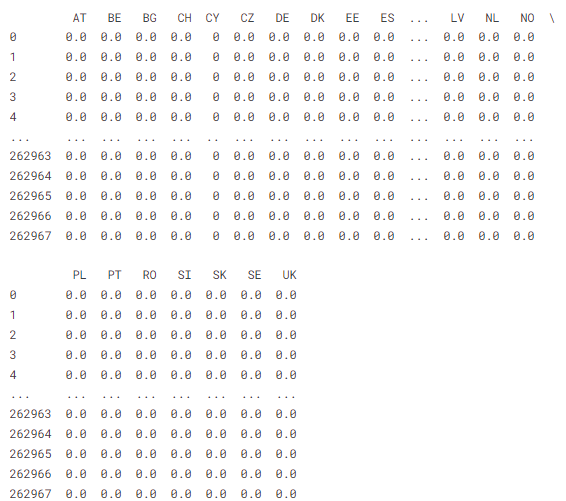
\includegraphics[width=0.8\linewidth]{EMHIRES Structure.png}
    \caption{EMHIRES dataset example}
    \label{fig:Fig1}
  \end{figure}

\subsection{Monthly Electricity Statistics}
The data contained in this dataset has been collected by the International Energy Agency (IEA) \cite{iea_data}.
These data include information on energy in various countries from 2010 to 2022.
Energy production is measured in gigawatt-hours (GWh) and covers various energy products, including solar energy.
You can get an idea of the structure of this dataset from Figure \ref{fig:Fig2}.

\begin{figure}[h]
    \centering
    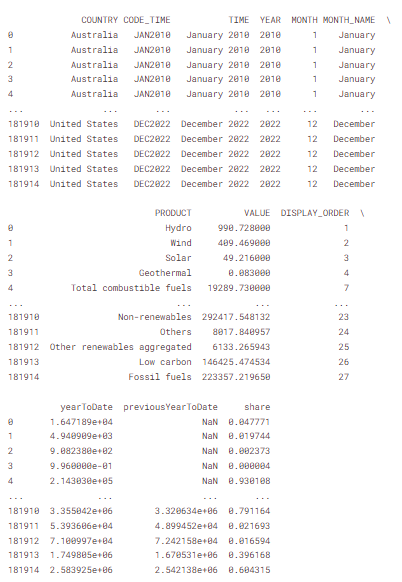
\includegraphics[width=0.5\linewidth]{IEA.png}
    \caption{IEA dataset example}
    \label{fig:Fig2}
\end{figure}

\subsubsection{Dataset Features}
The dataset contains various features, which are as follows:

\begin{description}[left=0pt, labelwidth=2.5cm, labelsep=1em, font=\normalfont]
    \item[\textbf{COUNTRY:}] Name of the country
    \item[\textbf{CODE\_TIME:}] A code representing the month and year (e.g., JAN2010 for January 2010)
    \item[\textbf{TIME:}] The month and year in a more human-readable format (e.g., January 2010)
    \item[\textbf{YEAR:}] The year of the data point
    \item[\textbf{MONTH:}] The month of the data point as a number (1-12)
    \item[\textbf{MONTH\_NAME:}] The month of the data point as a string (e.g., January)
    \item[\textbf{PRODUCT:}] The type of energy product (e.g., hydropower, wind, solar)
    \item[\textbf{VALUE:}] The amount of electricity generated in gigawatt-hours (GWh)
    \item[\textbf{DISPLAY\_ORDER:}] The order in which products should be displayed
    \item[\textbf{yearToDate:}] The amount of electricity generated for the current year up to the current month in GWh
    \item[\textbf{previousYearToDate:}] The amount of electricity generated for the previous year up to the current month in GWh
    \item[\textbf{share:}] The share of the product in the total electricity production for the country in decimal format
\end{description}

\subsubsection{Dataset Statistics}
IEA has compiled accessible statistics on the webpage \url{https://www.iea.org/data-and-statistics/data-tools/monthly-electricity-statistics}. These statistics provide a comprehensive overview of how energy production has changed over the years and offer detailed information on the most utilized renewable energy sources.
\\
It is evident that, in this historical period, solar energy is one of the prominent renewable energies, as can be observed by analyzing the data presented in the statistics. I do not include the images available on that website as the rights related to those graphics are reserved.

\section{Other Datasets}
The datasets previously presented are considered more "complete" and reliable as they have been published by European authorities or reputable companies. However, to conduct my study, I have also employed other datasets that may have less detailed or less reliable documentation. Despite this, I believe they are still correct since, upon analyzing the data, it is evident that they exhibit a certain degree of coherence. I will explain in more detail the reason for this choice later.

\subsection{World Weather Repository}
This dataset \cite{global-weather-repository} provides daily meteorological information for capitals worldwide. Unlike forecast data, this dataset offers a complete set of features reflecting current weather conditions globally. It started collecting data from August 29, 2023.
\\
The dataset includes over 40 features, including temperature, wind, pressure, precipitation, humidity, visibility, air quality measurements, and more. This extensive set of data is valuable for analyzing global meteorological patterns, exploring climate trends, and understanding relationships between different weather parameters.
\\
The dataset features are as follows:

\begin{multicols}{2}
\begin{itemize}
  \item \textbf{country:} Country of meteorological data
  \item \textbf{location\_name:} Name of the location (city)
  \item \textbf{latitude:} Latitude coordinate of the location
  \item \textbf{longitude:} Longitude coordinate of the location
  \item \textbf{timezone:} Timezone of the location
  \item \textbf{last\_updated\_epoch:} Unix timestamp of the last data update
  \item \textbf{last\_updated:} Local time of the last data update
  \item \textbf{temperature\_celsius:} Temperature in degrees Celsius
  \item \textbf{temperature\_fahrenheit:} Temperature in degrees Fahrenheit
  \item \textbf{condition\_text:} Description of weather conditions
  \item \textbf{wind\_mph:} Wind speed in miles per hour
  \item \textbf{wind\_kph:} Wind speed in kilometers per hour
  \item \textbf{wind\_degree:} Wind direction in degrees
  \item \textbf{wind\_direction:} Wind direction as a 16-point compass
  \item \textbf{pressure\_mb:} Pressure in millibars
  \item \textbf{pressure\_in:} Pressure in inches
  \item \textbf{precip\_mm:} Amount of precipitation in millimeters
  \item \textbf{precip\_in:} Amount of precipitation in inches
  \item \textbf{humidity:} Humidity in percentage
  \item \textbf{cloud:} Cloud cover in percentage
  \item \textbf{feels\_like\_celsius:} Feels-like temperature in degrees Celsius
  \item \textbf{feels\_like\_fahrenheit:} Feels-like temperature in degrees Fahrenheit
  \item \textbf{visibility\_km:} Visibility in kilometers
  \item \textbf{visibility\_miles:} Visibility in miles
  \item \textbf{uv\_index:} UV index
  \item \textbf{gust\_mph:} Wind gust in miles per hour
  \item \textbf{gust\_kph:} Wind gust in kilometers per hour
  \item \textbf{air\_quality\_Carbon\_Monoxide:} Air quality measurement: Carbon Monoxide
  \item \textbf{air\_quality\_Ozone:} Air quality measurement: Ozone
  \item \textbf{air\_quality\_Nitrogen\_dioxide:} Air quality measurement: Nitrogen Dioxide
  \item \textbf{air\_quality\_Sulphur\_dioxide:} Air quality measurement: Sulphur Dioxide
  \item \textbf{air\_quality\_PM2.5:} Air quality measurement: PM2.5
  \item \textbf{air\_quality\_PM10:} Air quality measurement: PM10
  \item \textbf{air\_quality\_us-epa-index:} Air quality measurement: US EPA Index
  \item \textbf{air\_quality\_gb-defra-index:} Air quality measurement: GB DEFRA Index
  \item \textbf{sunrise:} Local time of sunrise
  \item \textbf{sunset:} Local time of sunset
  \item \textbf{moonrise:} Local time of moonrise
  \item \textbf{moonset:} Local time of moonset
  \item \textbf{moon\_phase:} Current moon phase
  \item \textbf{moon\_illumination:} Percentage of moon illumination
\end{itemize}
\end{multicols}
You can see some rows of the dataset in Figure \ref{fig:combined}


\begin{figure}[h]
    \centering
    \begin{subfigure}{0.48\textwidth}
      \centering
      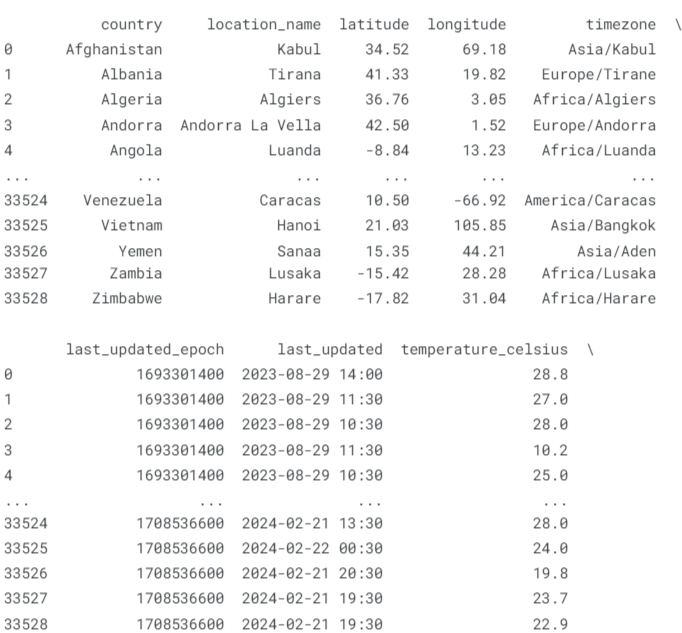
\includegraphics[width=\linewidth]{WWR.png}
      \label{fig:sub1}
    \end{subfigure}
    \hfill
    \begin{subfigure}{0.48\textwidth}
      \centering
      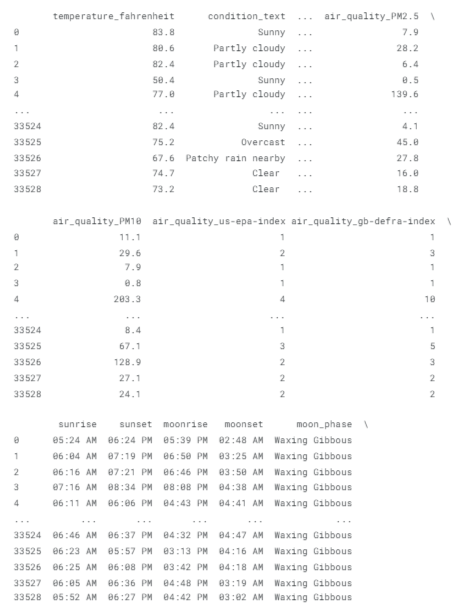
\includegraphics[width=\linewidth]{WWR2.png}
      \label{fig:sub2}
    \end{subfigure}
    \caption{World Weather Repository dataset example}
    \label{fig:combined}
  \end{figure}

\newpage
\subsection{Norway meteorological data}
The dataset \cite{Norway-Meteorological-Dataset} represents a collection of precompiled and pre-processed meteorological data obtained from the meteorologisk institutt archive in Oslo, Norway, through its Frost API (\url{https://frost.met.no/index.html}).
Data is collected from 55 meteorological stations distributed throughout Norway from January 1, 2010, to December 31, 2021. Each record in the dataset includes the station's identifier and geographical coordinates, date breakdown, and various observations such as maximum and average air temperature for the specific day, maximum and average wind speed, maximum relative humidity, and the sum of precipitation for the specific day. It's important to note that some values may be missing (\texttt{NaN}) as some stations only record some of the mentioned metrics.
\\
To ensure consistency and ease of use of the dataset, you can proceed with the removal of unnecessary or redundant information. Additionally, you can further expand the dataset by incorporating additional variables or metrics of interest for a specific study.
\\
The features present in this dataset are:
\begin{itemize}
    \item Unnamed: 0
    \item sourceId
    \item latitude
    \item longitude
    \item max(air\_temperature P1D)
    \item max(relative\_humidity P1D)
    \item max(wind\_speed P1D)
    \item mean(air\_temperature P1D)
    \item mean(relative\_humidity P1D)
    \item mean(wind\_speed P1D)
    \item sum(precipitation\_amount P1D)
    \item day
    \item month
    \item year
\end{itemize}

To see an example of how this dataset is structured, you can refer to Figure \ref{fig:combined2}

\begin{figure}[h]
    \centering
    \begin{subfigure}{0.48\textwidth}
      \centering
      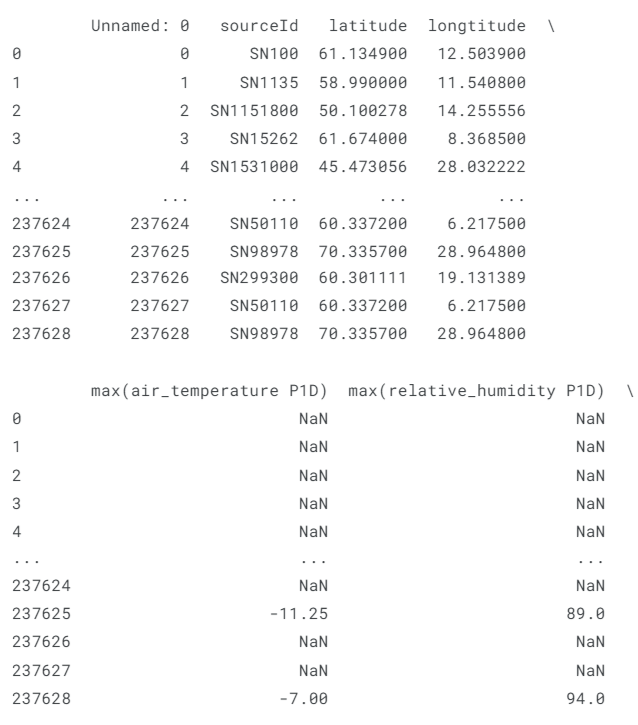
\includegraphics[width=\linewidth]{Nor1.png}
    \end{subfigure}
    \hfill
    \begin{subfigure}{0.48\textwidth}
      \centering
      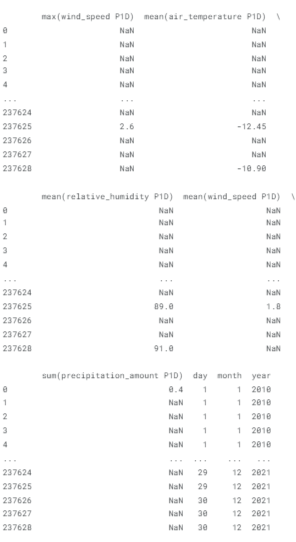
\includegraphics[width=\linewidth]{Nor2.png}
    \end{subfigure}
    \caption{Norway-Meteorological-Dataset dataset example}
    \label{fig:combined2}
  \end{figure}

  \section{Cleaning and Analysis}
  After a lengthy phase of identifying datasets, during which many were discarded from an initial group, I initiated the subsequent phase of cleaning and in-depth analysis (you can refer to the code \href{https://www.kaggle.com/code/alessandromajumba/small-project-in-ai}{here}).
  \\
  During this process, I carefully examined the datasets, identified the most relevant features, and addressed the handling of missing values, replacing them with appropriate values. Additionally, I observed the overall behavior of the datasets over time.
  \\
  A crucial aspect of my study was exploring the existence of any trends, particularly checking if there was a consistent increase in energy production during summer months compared to winter months. For this analysis, I created various visualizations. A result contradicting this expectation could indicate a potential issue with data quality.
  \\
  During this phase, I paid particular attention to ensuring the integrity and reliability of the data, aiming to obtain meaningful results for a correct interpretation of patterns and relationships in the datasets.
  \\
  Figures~\ref{fig:combined3} and~\ref{fig:combined4} clearly show how the graphs exhibit the expected behavior.

\newpage
\begin{figure}[h]
    \centering
    \begin{subfigure}{0.48\textwidth}
      \centering
      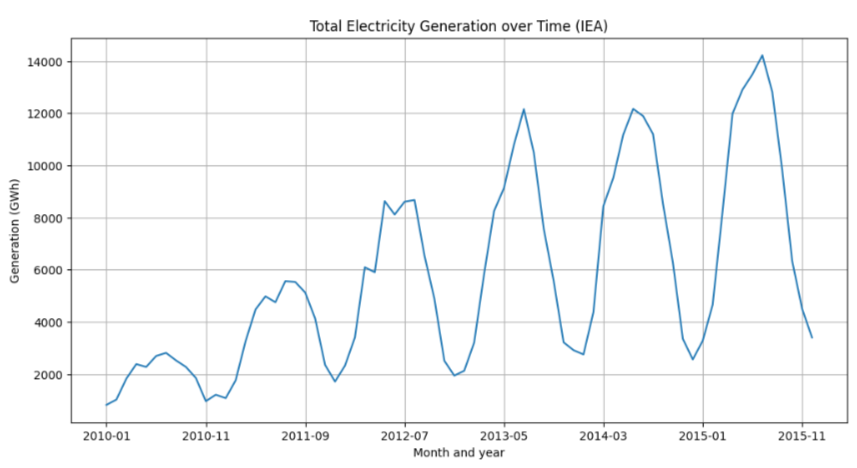
\includegraphics[width=\linewidth]{IEA Graph.png}
    \end{subfigure}
    \hfill
    \begin{subfigure}{0.48\textwidth}
      \centering
      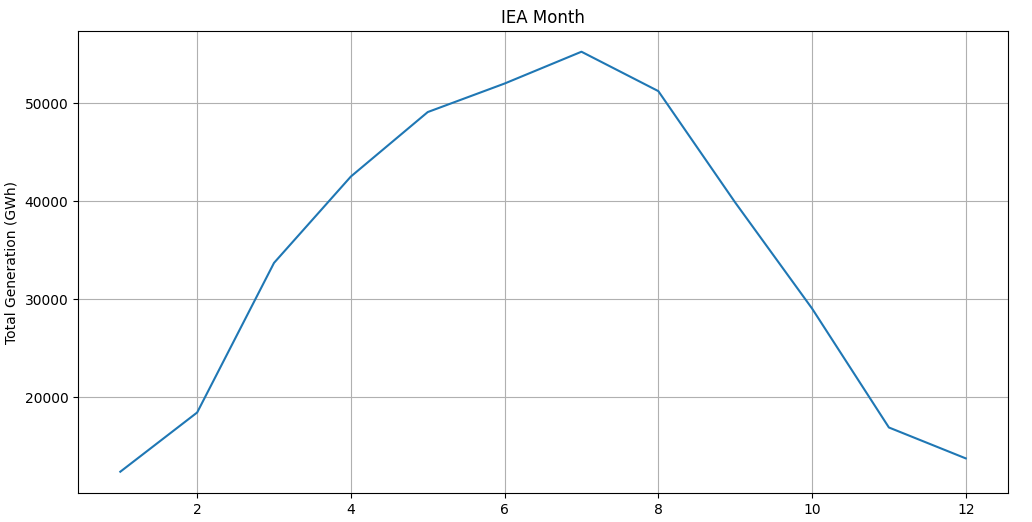
\includegraphics[width=\linewidth]{IEA Graph2.png}
    \end{subfigure}
    \caption{IEA plot}
    \label{fig:combined3}
  \end{figure}

  \begin{figure}[h]
    \centering
    \begin{subfigure}{0.48\textwidth}
      \centering
      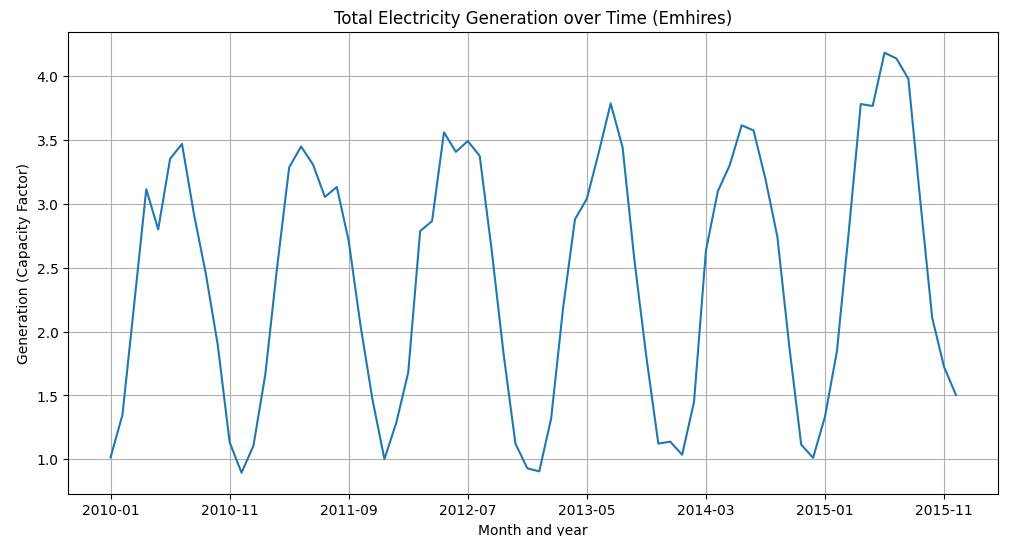
\includegraphics[width=\linewidth]{EMHIRES Graph.png}
    \end{subfigure}
    \hfill
    \begin{subfigure}{0.48\textwidth}
      \centering
      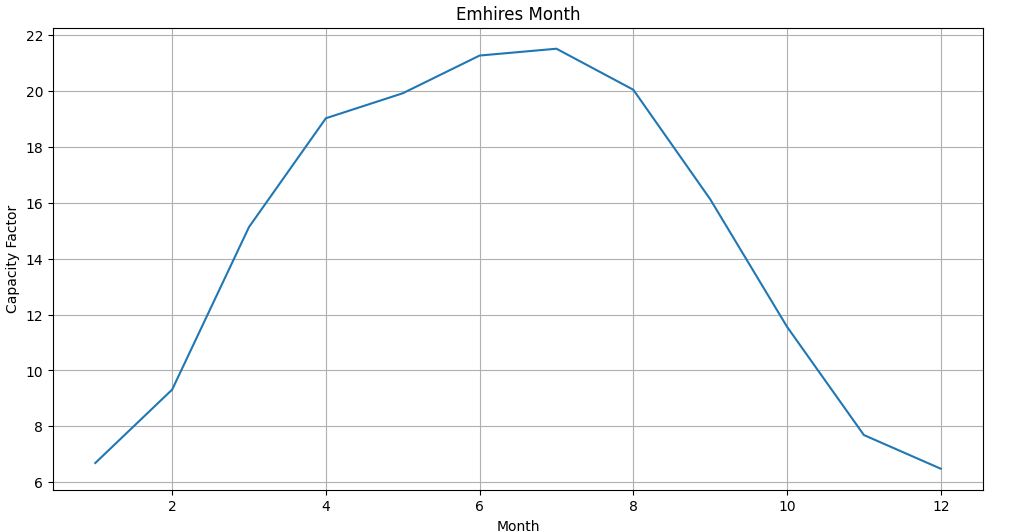
\includegraphics[width=\linewidth]{EMHIRES Graph2.png}
    \end{subfigure}
    \caption{EMHIRES plot}
    \label{fig:combined4}
\end{figure}

\clearpage
\section{Models}
\subsection{EMHIRES Model}
After completing the phase of studying and cleaning the datasets, I proceeded with the development of regression models. I started using the EMHIRES dataset, and the code is available \href{https://www.kaggle.com/code/alessandromajumba/model-emhires}{EMHIRES Model}.
\\
After an initial data pre-processing phase, I created several regression models, starting with simpler approaches and gradually advancing to more complex models, such as Recurrent Neural Networks (RNN). The EMHIRES dataset is of considerable size, allowing for good performance even with a limited number of epochs.
\\
After training, I managed to achieve the following results:

\begin{itemize}
  \item \texttt{Training Loss: 0.03785869851708412}
  \item \texttt{Validation Loss: 0.03948716109068664}
  \item \texttt{Test Loss: 0.03929314762353897}
\end{itemize}

These values are quite good and indicate that the model has adapted satisfactorily to the data.

\subsection{IEA Monthly Electricity Statistics}
For the IEA dataset, I followed the same process as described earlier (\href{https://www.kaggle.com/code/alessandromajumba/iea-model}{IEA Code}). Initially, I performed a preprocessing phase on the dataset, including normalization, removal of unnecessary features, and one-hot encoding. Subsequently, I created a regression model using an RNN. Since the dataset is significantly smaller than the previous one, I used a higher number of epochs during training.

After the training phase, I obtained the following results for the loss metrics:

\begin{itemize}
    \item \texttt{Training Loss: 0.012684706598520279}
    \item \texttt{Validation Loss: 0.14131624661014952}
    \item \texttt{Test Loss: 0.08876131474971771}
\end{itemize}

These values indicate that the model has adapted satisfactorily to the data.

I also calculated some model evaluation metrics:

\begin{itemize}
    \item \textbf{R-squared (r2):} Represents the proportion of variance explained by the model, obtaining a value of \texttt{0.9294676281171568}, indicating good predictive ability.
    \item \textbf{Mean Squared Error (MSE):} Measures the average of the squared errors and is \texttt{0.07650821274623916}.
    \item \textbf{Mean Absolute Error (MAE):} Represents the average of absolute errors and has a value of \texttt{0.20185678746688712}.
\end{itemize}

These metrics reflect good accuracy of the model in predicting IEA dataset's data. The high R-squared value suggests that a significant portion of the variance is explained by the model, and the low MSE and MAE values indicate good adaptability to the data.

\subsection{Mixed Model}
After training the main datasets, it was decided to also consider day and night hours to check if adding information about sunrise and sunset times could lead to more accurate performance. To test this hypothesis, I combined the IEA Dataset with the World Weather Repository (which contains sunrise and sunset times for some countries, and you can find the code \href{https://www.kaggle.com/code/alessandromajumba/iea-model-world-weather-repository}{here}).
\\
I focused only on the country "Austria" since the World Weather Repository dataset does not contain all the countries present in the IEA dataset. However, it is reasonable to assume that if better values are obtained for one country, the same reasoning can be extended to all the other available countries.
\\
From Figure \ref{fig:merged}, you can see how the dataset looks after merging and eliminating non-significant columns.
\\
On this dataset, I performed one-hot encoding for the dates and then proceeded to train the model.
\\
The obtained metrics are as follows (with the same model parameters):
\begin{itemize}
    \item \texttt{Training Loss: 0.0004668822803068906 (Figure \ref{fig:TC})}
    \item \texttt{Validation Loss: 0.021887180635916294 (Figure \ref{fig:vC})}
    \item \texttt{Test Loss: 0.08139250427484512}
    \item \texttt{R-squared (r2): 0.9135166954729765}
    \item \texttt{Mean Squared Error (MSE): 0.08139250993211926} 
    \item \texttt{Mean Absolute Error (MAE): 0.22941606556120853}
\end{itemize}

\begin{figure}[h]
  \centering
  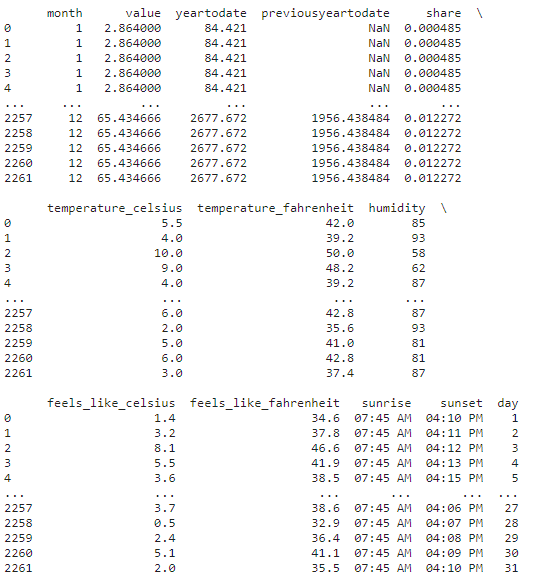
\includegraphics[width=0.5\linewidth]{Merged_df.png}
  \caption{IEA +  World Weather Repository dataset example}
  \label{fig:merged}
\end{figure}

\begin{figure}[h]
    \centering
    \begin{subfigure}{0.6\textwidth}
      \centering
      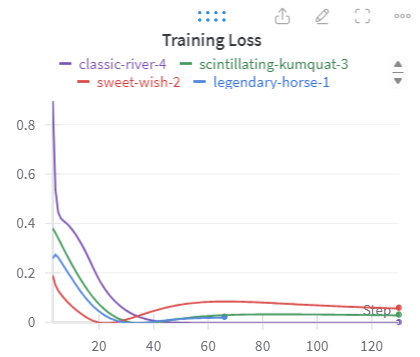
\includegraphics[width=0.9\linewidth]{Training 3.png}
      \caption{Training Curves}
      \label{fig:TC}
    \end{subfigure}
    \hfill
    \begin{subfigure}{0.6\textwidth}
      \centering
      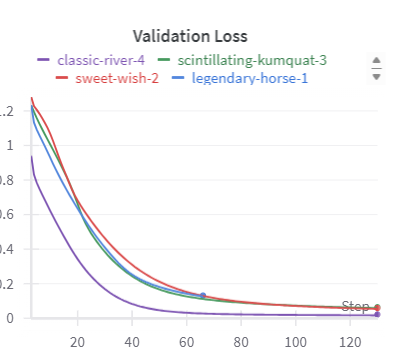
\includegraphics[width=0.9\linewidth]{Validation3.png}
      \caption{Validation Curves}
      \label{fig:vC}
    \end{subfigure}
    \caption{Curves}
    \label{fig:combined5}
\end{figure}


These are slightly better parameters than those obtained previously.


\newpage
\section{Conclusion}
This work addresses the significant issue of solar energy prediction, currently a topic of great interest in the energy industry. A considerable portion of the work focused on identifying and correcting datasets. Finding reliable datasets from official sources, containing data over a long period, proved to be a significant challenge.
\\
In the process of identifying datasets, crucial questions emerged: what can we do with these data? Do we need to modify some features? Are the datasets complete? Do they make sense when considered together over an extended period?
\\
Numerous datasets did not satisfactorily answer these questions, and for this reason, they were discarded and not included in this study. The next phase of the work involved creating models based on the identified datasets. These models naturally had to make predictions. The main challenge was to identify the model that best fit the data, ensuring a good balance between performance and training time.
\\
Further complications arose when exploring the effectiveness of combining different datasets, containing information beyond energy production, such as sunrise and sunset times and meteorological phenomena. A specific study conducted for Austria indicated a slight but significant improvement in performance.
\\
Future developments of the project could involve the search for additional data that, combined with the already available ones, allow for more accurate predictions. Features such as cloud presence throughout the year, advanced meteorological details, and climate changes could be considered to further improve prediction accuracy.

\clearpage
\printbibliography

\end{document}



